\chapter{Valorisation}
\label{sec:valor}
\setstretch{\lspac}

According to the regulation governing the attainment of doctoral degrees at Uni\-versi\-teit Maas\-tricht, an addendum about valorisation must be added to each doctoral thesis. This is the purpose of this section. Note that each of the previous chapters has its own conclusion.

\section{Introduction}

Before this work, there was a considerable confusion on what would be the proper way of studying the surface area of the cerebral cortex at a finer scale, across subjects, with many improvised approaches having appeared. None of these, however had sufficiently considered the deleterious impact that non-pycnophylactic methods would have on measurements. The work presented in Chapter~\ref{sec:areal} provided a much missed ground truth to which other, possibly faster even if approximate, strategies can be compared.

While the study of surface area is definitely not the only one to benefit from permutation inference, it is one where such non-parametric techniques can be applied in their whole potential, for providing robust inference even when assumptions about normality do not hold, and allowing correction for multiplicity of tests in spite of the complex dependence structure and irregular lattice of facewise areal data. The investigation of various regression and permutation strategies provided in Chapter~\ref{sec:perm}, allied with the use of exchangeability blocks, variance groups, permutations together with sign-flippings, and a statistic that is robust to heteroscedasticity, the $G$-statistic, allows researchers to use permutation tests confidently even with complex designs.

For multimodal data, and for unexplored, yet pervasive types of multiple testing, the non-parametric combination (\textsc{npc}) framework provided in Chapter~\ref{sec:comb} compares favourably against classical multivariate tests, such as \textsc{mancova}, with power that grows intuitively and consistently with the inclusion of data that truly contains the effect being sought. The \textsc{npc} allows the analysis of cortical gray matter volume from surface-based methods, even when its separate constituent parts have possibly cancelling effects on each other.

\section{Thesis impact}

The most obvious impact of this thesis is that it provided:

\begin{itemize}
\item[--] A method to study the surface area of the cortex, of populations of subjects, at a fine resolution.
\item[--] A thorough investigation of permutation tests in the presence of nuisance variables.
\item[--] Assessment of permutations with sign flippings.
\item[--] Whole-block and within-block permutation.
\item[--] A heteroscedasticity-robust test statistic.
\item[--] A version of \textsc{npc} that is feasible for neuroimaging applications.
\item[--] A demonstration of the superior power of \textsc{npc} when compared to classical tests.	
\end{itemize}

\subsection{Peer-reviewed publications}

\begin{itemize}
\item[--] Winkler AM, Sabuncu MR, Yeo BT, Fischl B, Greve DN, Kochunov P, Nichols TE, Blangero J, Glahn DC. Measuring and comparing brain cortical surface area and other areal quantities. \emph{NeuroImage}. 2012 Mar 15;61(4):1428-43.
\item[--] Winkler AM, Ridgway GR, Webster MA, Smith SM, Nichols TE. Permutation inference for the general linear model. \emph{NeuroImage}. 2014 May 15;92:381-97.
\item[--] Winkler AM, Webster MA, Brooks JC, Tracey I, Smith SM and Nichols TE. Non-parametric combination and related permutation tests for neuroimaging. \emph{Human Brain Mapping}. 2016 (\emph{in press}).
\end{itemize}

\subsection{Presentations in conferences}

\begin{itemize}
\item[--] Winkler AM, Sabuncu MR, Yeo BT, Fischl B, Greve DN, Kochunov P, Nichols TE, Blangero J, Glahn DC. \emph{Measuring and comparing brain cortical surface area and other areal quantities}. 18th Human Brain Mapping, 10-14 June 2012, Beijing, China.
\item[--] Winkler AM, Smith SM, Nichols TE. \emph{Non-parametric combination for analyses of multi-modal imaging}. 19th Human Brain Mapping, 16-20 June 2013, Seattle, WA, USA; also presented at: Neuroimaging Data Analysis. Statistical and Applied Mathematical Sciences Institute (\textsc{samsi}), 04-14 June 2013, Research Triangle Park, North Carolina, \textsc{usa}.
\item[--] Winkler AM, Ridgway GR, Webster MA, Smith SM, Nichols TE. \emph{Permutation inference for the general linear model and the $G$-statistic}. 20th Human Brain Mapping, 8-12 June 2014, Hamburg, Germany.
\end{itemize}

\subsection{Talks}

\begin{itemize}
\item[--] \emph{Areal analysis}. Talk at the \textsc{fmrib} Analysis Group meeting, 13 February 2013, University of Oxford, \textsc{uk}.
\item[--] \emph{Permutation for the general linear model}. Talk at at the Department of Statistics, University of Warwick, \textsc{uk}, on 27 March 2014.
\item[--] \emph{Permutation for the general linear model}. This was a series of three talks delivered in 3, 10 and 17 September 2015 at \textsc{fmrib}, University of Oxford, \textsc{uk}. The talks covered permutation for the general linear model, block permutation, multivariate methods (classical \textsc{manova}, etc), non-parametric combination for brain imaging data (\textsc{npc}), and multi-level block permutation, therefore including topics beyond those covered in this dissertation.
\item[--] \emph{Areal and volumetric analyses}. Talk at the Department of Laboratory Medicine, Children’s and Women’s Health, 14 April 2015, Norwegian University of Science and Technology, Trondheim, Norway.

\end{itemize}

\subsection{Public engagement}

Various small pieces of information that were studied during the development of this dissertation have been published in the blog of the author: \href{http://brainder.org}{brainder.org}. This includes entries about normality tests, the Box--Cox transformation and log\-normality, quality inspection of results of FreeSurfer surface reconstruction, vertexwise and facewise file formats, confidence intervals for Bernoulli trials, biases on permutation p-values, the logic of the method of Fisher to combine p-values, the classic ``lady tasting tea'' experiment (a form of permutation test), among others. Scripts for areal analyses, for smoothing quickly vertexwise or facewise data after interpolation to a regular mesh, to generate a regular spherical mesh, and for visualisation of areal quantities (facewise) are also provided in the blog.

\subsection{Software}

Scripts for areal interpolation, smoothing, conversion from facewise to vertexwise, and facewise data visualisation, as presented in Chapter~\ref{sec:areal}, have been made available, and can be obtained from \href{http://brainder.org}{brainder.org}. The permutation tests, as discussed in Chapters \ref{sec:perm} and \ref{sec:comb}, have been made available in the tool \emph{Permutation Analysis of Linear Models} (\textsc{palm}), a text-based application that can be invoked from scripts, and that can be downloaded from \href{http://fsl.fmrib.ox.ac.uk/fsl/fslwiki/PALM}{fsl.fmrib.ox.ac.uk/fsl/fslwiki/\textsc{palm}} (Figure~\ref{fig:valor:palm}). It should be noted, however, that \textsc{palm} includes various other features that are not covered by this dissertation. Both \textsc{palm} and the scripts for areal analysis are licensed under the General Public Licence (\textsc{gpl}), thus can be distributed freely, and run in either \textsc{Matlab} or Octave.

\begin{figure}[tbp]
\begin{center}
\centerline{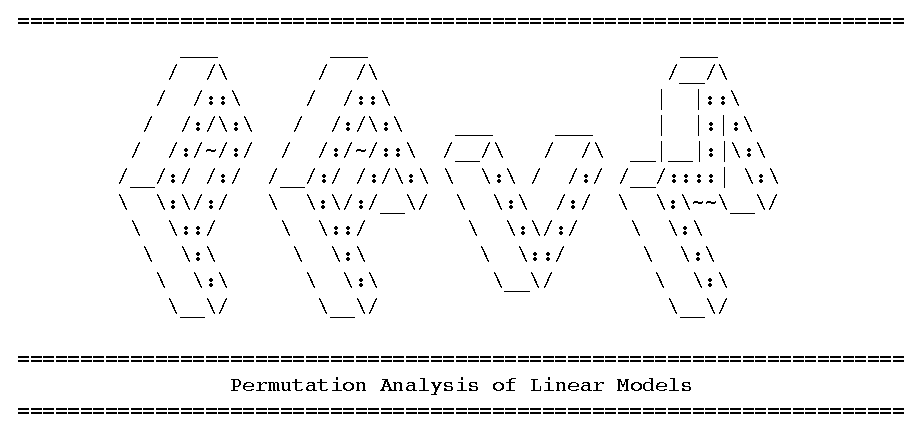
\includegraphics[width=12cm]{images/palm.eps}}
\end{center}
\caption[The proposed tests are available in \textsc{palm}.]{The permutation tests discussed and proposed in Chapters \ref{sec:perm} and \ref{sec:comb} have been made available in the tool \emph{Permutation Analysis of Linear Models} (\textsc{palm}), a text-based application that can be invoked from scripts.}
\label{fig:valor:palm}
\end{figure}

\section{Further perspectives}

The work in this thesis has already unfolded into rich consequences. The whole-block and within-block exchangeability can be nested into each other, so as to allow multi-level exchangeability blocks, a work that the author has already developed as a side-project, and that is already published \citep{Winkler2015}.

While the pycnophylactic interpolation is clearly the most appropriate way of assessing area, it is computationally demanding given the high resolution of the cortical meshes typically used, and an assessment of other, approximate methods, is necessary so as to reduce computational costs. In the same line, permutation tests are much slower than their parametric counterparts. Strategies for acceleration should to be considered if these methods are to be used for routine analysis.

Finally, the demonstration that permutation tests can be used in complex experimental designs as those considered opens up many possibilities, particularly for the analysis of multi-level \textsc{fmri} data, as well as for cases in which not all observations are present. This includes cases that currently can only be treated with linear mixed effects models, which has all the disadvantages inherent to iterative methods.